\documentclass{article}
\usepackage[utf8]{inputenc}

\title{LOC ERROR}
\author{ }
\date{May 2016}

\usepackage{natbib}
\usepackage{graphicx}
\usepackage{multirow}

\begin{document}

\maketitle

\section{Introduction}
There is a theory which states that if ever anyone discovers exactly what the Universe is for and why it is here, it will instantly disappear and be replaced by something even more bizarre and inexplicable.
There is another theory which states that this has already happened.


\begin{table}[!htpb]
\centering
\caption{NASA10}
\label{tab:nasa10}
\begin{tabular}{|r|c|c|c|c|}
\hline
\multicolumn{1}{|c|}{\multirow{2}{*}{\textbf{Name}}} & \multicolumn{2}{c|}{\textbf{Mean}}     & \multicolumn{2}{c|}{\textbf{Variance}} \\ \cline{2-5} 
\multicolumn{1}{|c|}{}                               & \textbf{Rank} & \textbf{Med $\pm$ IQR} & \textbf{Rank} & \textbf{Med $\pm$ IQR} \\ \hline
COCOMO2                                              & 1             & 43 $\pm$ 35            & 1             & 0 $\pm$ 0              \\
0.2:COCOMO2                                          & 1             & 38 $\pm$ 32            & 1             & 1 $\pm$ 1              \\ \cline{4-5}
0.4:COCOMO2                                          & 1             & 45 $\pm$ 40            & 2             & 2 $\pm$ 2              \\ \cline{2-3}
0.6:COCOMO2                                          & 2             & 49 $\pm$ 30            & 2             & 4 $\pm$ 2              \\ \cline{4-5}
0.8:COCOMO2                                          & 2             & 49 $\pm$ 36            & 3             & 6 $\pm$ 3              \\
1.0:COCOMO2                                          & 2             & 50 $\pm$ 34            & 3             & 8 $\pm$ 7    \\ \hline         
\end{tabular}
\end{table}

% Please add the following required packages to your document preamble:
% \usepackage{multirow}
\begin{table}[!htpb]
\centering
\caption{COC05}
\label{tab:coc05}
\begin{tabular}{|r|c|c|c|c|}
\hline
\multicolumn{1}{|c|}{\multirow{2}{*}{\textbf{Name}}} & \multicolumn{2}{c|}{\textbf{Mean}}     & \multicolumn{2}{c|}{\textbf{Variance}} \\ \cline{2-5} 
\multicolumn{1}{|c|}{}                               & \textbf{Rank} & \textbf{Med $\pm$ IQR} & \textbf{Rank} & \textbf{Med $\pm$ IQR} \\ \hline
COCOMO2                                              & 1             & 46 $\pm$ 134           & 1             & 0 $\pm$ 0              \\ \cline{4-5}
0.2:COCOMO2                                          & 1             & 46 $\pm$ 132           & 2             & 2 $\pm$ 9              \\ \cline{4-5}
0.4:COCOMO2                                          & 1             & 48 $\pm$ 131           & 3             & 5 $\pm$ 36             \\
0.6:COCOMO2                                          & 1             & 50 $\pm$ 120           & 3             & 8 $\pm$ 80             \\ \cline{4-5}
0.8:COCOMO2                                          & 1             & 63 $\pm$ 100           & 4             & 12 $\pm$ 130           \\
1.0:COCOMO2                                          & 1             & 65 $\pm$ 113           & 4             & 18 $\pm$ 162 \\ \hline
\end{tabular}
\end{table}


% Please add the following required packages to your document preamble:
% \usepackage{multirow}
\begin{table}[!htpb]
\centering
\caption{NASA93}
\label{tab:nasa93}
\begin{tabular}{|r|c|c|c|c|}
\hline
\multicolumn{1}{|c|}{\multirow{2}{*}{\textbf{Name}}} & \multicolumn{2}{c|}{\textbf{Mean}}     & \multicolumn{2}{c|}{\textbf{Variance}} \\ \cline{2-5} 
\multicolumn{1}{|c|}{}                               & \textbf{Rank} & \textbf{Med $\pm$ IQR} & \textbf{Rank} & \textbf{Med $\pm$ IQR} \\ \hline
COCOMO2                                              & 1             & 39 $\pm$ 39            & 1             & 0 $\pm$ 0              \\
0.2:COCOMO2                                          & 1             & 39 $\pm$ 36            & 1             & 1 $\pm$ 1              \\ \cline{4-5}
0.4:COCOMO2                                          & 1             & 40 $\pm$ 33            & 2             & 2 $\pm$ 1              \\ \cline{4-5}
0.6:COCOMO2                                          & 1             & 42 $\pm$ 26            & 3             & 3 $\pm$ 3              \\ \cline{2-5}
0.8:COCOMO2                                          & 2             & 44 $\pm$ 23            & 4             & 6 $\pm$ 3              \\
1.0:COCOMO2                                          & 2             & 51 $\pm$ 18            & 4             & 8 $\pm$ 3          \\ \hline   
\end{tabular}
\end{table}


% Please add the following required packages to your document preamble:
% \usepackage{multirow}
\begin{table}[!htpb]
\centering
\caption{COC81}
\label{tab:coc81}
\begin{tabular}{|r|c|c|c|c|}
\hline
\multicolumn{1}{|c|}{\multirow{2}{*}{\textbf{Name}}} & \multicolumn{2}{c|}{\textbf{Mean}}     & \multicolumn{2}{c|}{\textbf{Variance}} \\ \cline{2-5} 
\multicolumn{1}{|c|}{}                               & \textbf{Rank} & \textbf{Med $\pm$ IQR} & \textbf{Rank} & \textbf{Med $\pm$ IQR} \\ \hline
COCOMO2                                              & 1             & 32 $\pm$ 33            & 1             & 0 $\pm$ 0              \\
0.2:COCOMO2                                          & 1             & 32 $\pm$ 32            & 1             & 1 $\pm$ 1              \\ \cline{4-5}
0.4:COCOMO2                                          & 1             & 36 $\pm$ 28            & 2             & 2 $\pm$ 3              \\ \cline{2-5}
0.6:COCOMO2                                          & 2             & 43 $\pm$ 15            & 3             & 4 $\pm$ 3              \\ \cline{2-3}
0.8:COCOMO2                                          & 3             & 49 $\pm$ 23            & 3             & 6 $\pm$ 5              \\ \cline{4-5}
1.0:COCOMO2                                          & 3             & 50 $\pm$ 19            & 4             & 9 $\pm$ 5      \\ \hline       
\end{tabular}
\end{table}


\begin{figure}
    \centering
    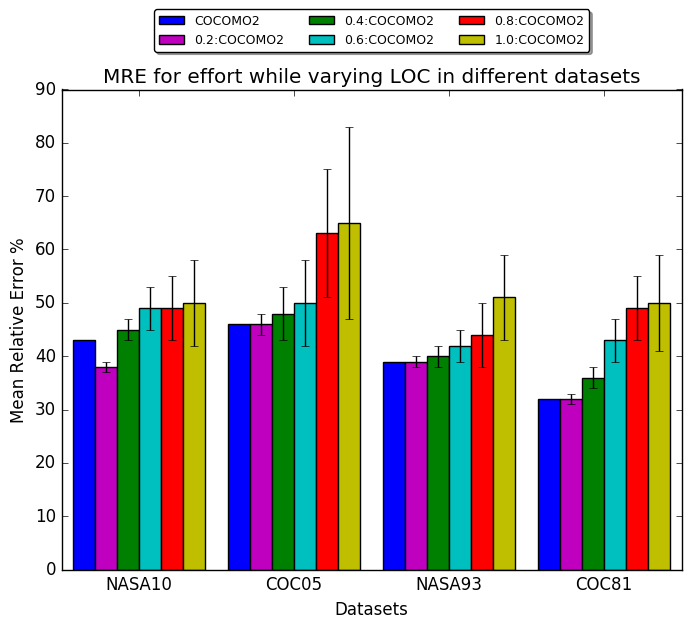
\includegraphics[scale=0.5]{Figs/mre.png}
    \caption{MRE for effor while varying LOC in different datasets.}
    \label{fig:mre_datasets}
\end{figure}

\section{Conclusion}
``I always thought something was fundamentally wrong with the universe'' \citep{adams1995hitchhiker}

\bibliographystyle{plain}
\bibliography{references}
\end{document}
